


\begin{figure}
    \centering
    \begin{subfigure}[tb]{0.48\textwidth}
        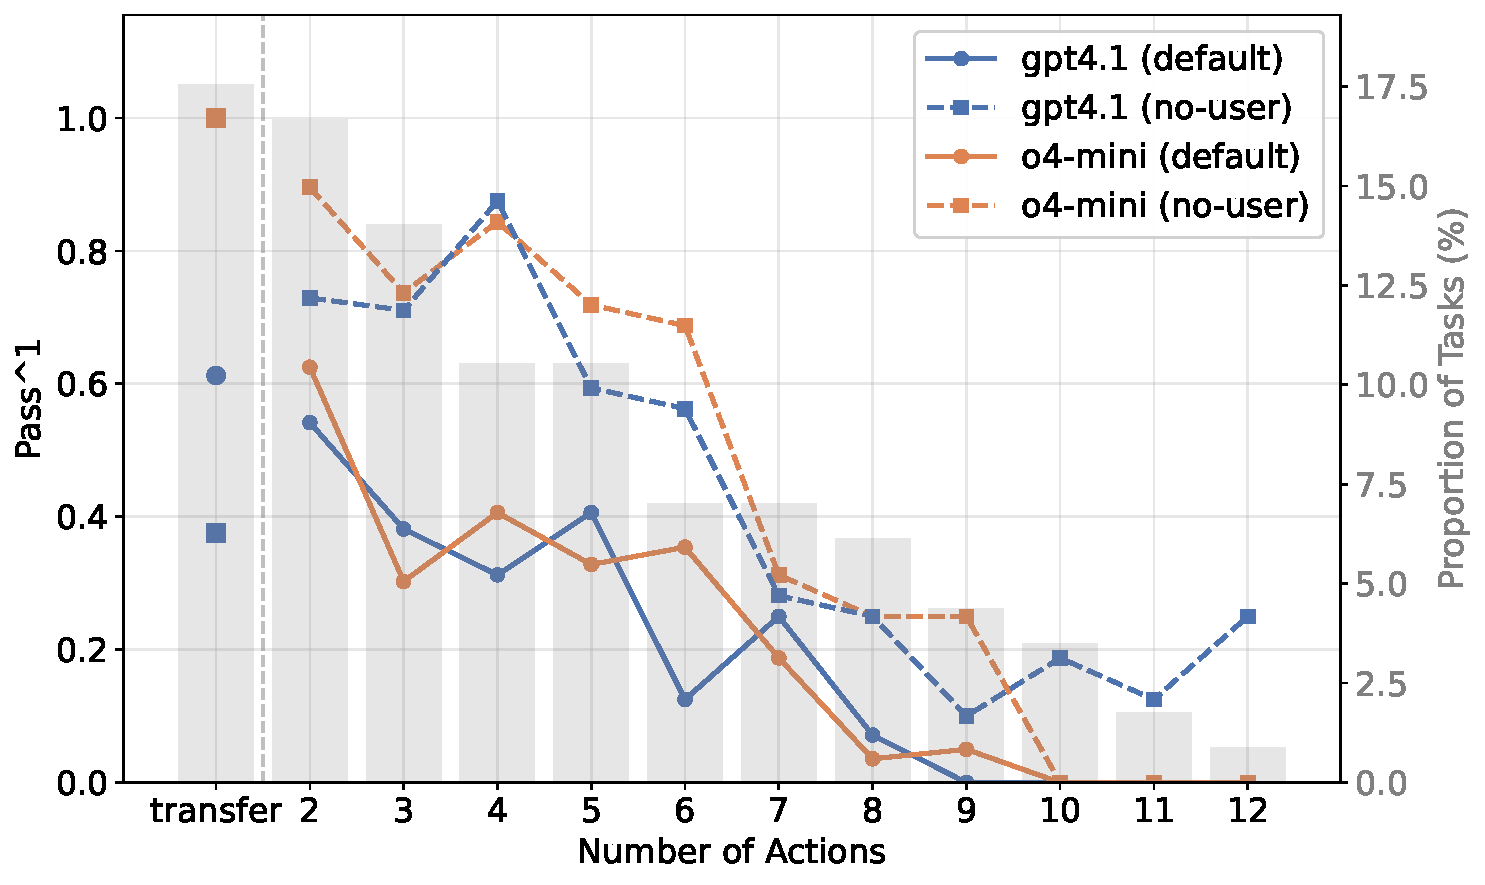
\includegraphics[width=\textwidth]{figures/results/pass_k_vs_num_actions_telecom_all_modes_llm_comparison.pdf}
    \end{subfigure}
    \hfill
    \begin{subfigure}[tb]{0.48\textwidth}
        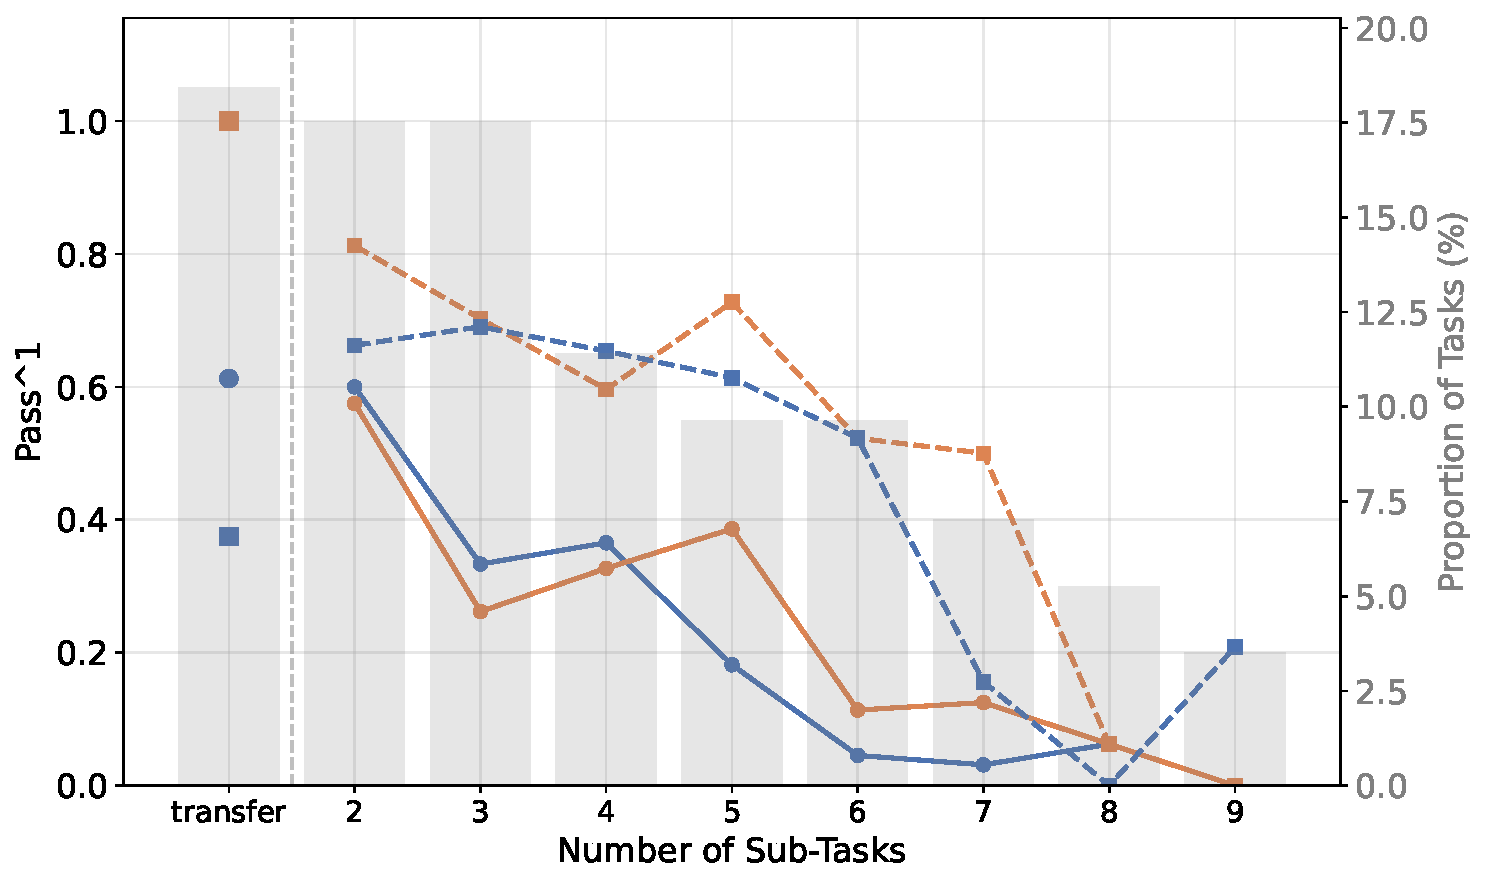
\includegraphics[width=\textwidth]{figures/results/pass_k_vs_num_issues_telecom_all_modes_llm_comparison.pdf}
    \end{subfigure}
    \vspace{-0.5em}
    \caption{\passone scores across various tasks in \telecom binned by the number of actions required to solve them (left) or the number of different issues that need to be addressed (right). \textit{transfer} refers to the special case of a task that requires to be transferred to a human and cannot be solved by the agent alone. (Grey bars indicates the proportion of the tasks that fall into that bin.)}
    \label{fig:telecom_results}
\end{figure}


